\chapter{Methods}
\label{c:methods}

\section{Methodological framework}
\label{s:methods:framework}

\todoparagraph{Explain what are the methods to be followed in the thesis and present it as a generic assessment platform/framework.}

\begin{figure}[h]
\centering
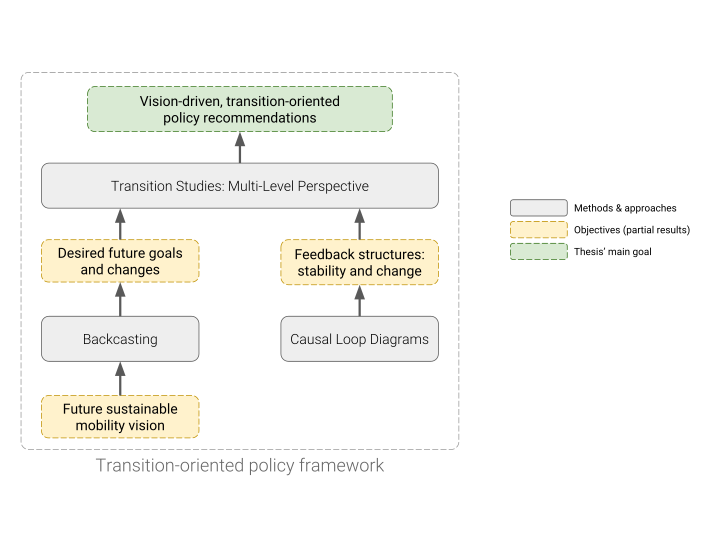
\includegraphics[trim=1cm 2cm 1.5cm 3cm,clip,width=\linewidth]{figures/methods-goals.pdf}
\caption[Thesis' methodological framework]{The generic methodological framework of the thesis. Note that the CLD model could be substituted by any other modelling technique which was sufficiently able to easily convey knowledge and insights to the key stakeholders and decision makers in the system.}
\label{fig:thesis-aim-methods}
\end{figure}

\todonote{Rephrase this!}The combination of assessment and planning tools, embedded in the discourse of transition studies, is used to discuss possible global patterns of development, by means of a dual backcasting and forecasting approach: scenario backcasting on one hand and system dynamics modelling on the other.

\section{Assumptions}
\label{s:methods:assumptions}

\todoparagraph{Explain what are the main assumptions and limitations of the proposed methodology -- for example, which is the normative perspective. Is the study normative? In which way is it? Are there data assumptions? Is there assumptions on the future development of the world? (scenarios, etc.)}

\subsection{Normative assumption}
\label{ss:methods:normative-assumption}

Following \textcite{creutzig2015_EvolvingNarrativesLow}, the normative assumption for the current study is made explicit, in order to clearly state the position and point of view of the author, as well as to ease the comparison to other studies and the reconciliation of the results with other approaches.

\todoparagraph{What is the normative assumption? Possibilities: \textit{liberal} or \textit{welfarist}, according to Creutzig (2015). Alternative: \textit{modular assessment} model.}